\documentclass[16pt]{article}
 
% Preamble

\usepackage[margin=22mm]{geometry}
\usepackage{amsfonts, amsmath, amssymb}
\usepackage{fancyhdr, float, graphicx}
\usepackage[utf8]{inputenc} % Required for inputting international characters
\usepackage[T1]{fontenc} % Output font encoding for international characters
\usepackage{fouriernc} % Use the New Century Schoolbook font
\usepackage[nottoc, notlot, notlof]{tocbibind}
\usepackage{listings}
\usepackage{xcolor}

\definecolor{codegreen}{rgb}{0,0.6,0}
\definecolor{codegray}{rgb}{0.5,0.5,0.5}
\definecolor{codepurple}{rgb}{0.58,0,0.82}
\definecolor{backcolour}{rgb}{0.95,0.95,0.92}

\lstdefinestyle{mystyle}{
    backgroundcolor=\color{backcolour},   
    commentstyle=\color{codegreen},
    keywordstyle=\color{magenta},
    numberstyle=\tiny\color{codegray},
    stringstyle=\color{codepurple},
    basicstyle=\ttfamily\footnotesize,
    breakatwhitespace=false,         
    breaklines=true,                 
    captionpos=b,                    
    keepspaces=true,                 
    numbers=left,                    
    numbersep=5pt,                  
    showspaces=false,                
    showstringspaces=false,
    showtabs=false,                  
    tabsize=2
}
\lstset{style=mystyle}

% \usepackage{url}
% \usepackage[options]{karnaugh-map}
% \usepackage{luacode}
% Header and Footer
\pagestyle{fancy}
\fancyhead{}
\fancyfoot{}
\fancyhead[L]{\textit{\Large{Project Report}}}
\fancyhead[R]{\textit{PP}}
\fancyfoot[C]{\thepage}
\renewcommand{\footrulewidth}{1pt}

% Other Doc Editing
% \parindent 0ex
%\renewcommand{\baselinestretch}{1.5}

\begin{document}

\begin{titlepage}
	\centering

	%---------------------------NAMES-------------------------------

	\huge\textsc{
		MIT World Peace University
	}\\

	\vspace{1\baselineskip} % space after Uni Name

	\LARGE{
		PYTHON PROGRAMING \\
		Second Year B.Tech, Semester 2
	}

	\vfill % space after Sub Name

	%--------------------------TITLE-------------------------------

	% \rule{\textwidth}{1.6pt}\vspace*{-\baselineskip}\vspace*{2pt}
	% \rule{\textwidth}{0.6pt}
	\vspace{3\baselineskip} % Whitespace above the title



	\huge{\textsc{
            PUzzlelists 
    }} \\



	% \vspace{0.5\baselineskip} % Whitespace below the title
	% \rule{\textwidth}{0.6pt}\vspace*{-\baselineskip}\vspace*{2.8pt}
	% \rule{\textwidth}{1.6pt}

	\vspace{7\baselineskip} % Whitespace after the title block

	%--------------------------SUBTITLE --------------------------	

	\LARGE\textsc{
		Project Report
			} % Subtitle or further description
	\vfill

	%--------------------------AUTHOR-------------------------------

	Prepared By
	\vspace{0.5\baselineskip} % Whitespace before the editors

	\Large{
		PA15. Parth Zarekar\\
        PA20. Krishnaraj Thadesar\\
		\vspace{1cm}
		Batch A1
	}


	\vspace{0.5\baselineskip} % Whitespace below the editor list
	\today

\end{titlepage}

\clearpage

\tableofcontents

\clearpage

\section{Introduction:}
Puzzelist is a Python-based game arcade that includes five popular games: Space Wars, Tetris, Snake, Icy, and 2048. The interface for Puzzelist is built using the PyQT library, which provides a user-friendly and interactive experience. In addition, Puzzelist also features a database to store user information, game scores, and the games that the user has unlocked. The purpose of this project is to showcase the versatility and fun of Python by creating an engaging game arcade that can be enjoyed by users of all ages.

\section{Problem Statement:}
The goal of Puzzelist is to provide a variety of games in a single platform that are easy to play and challenging enough to keep the users engaged. The challenge is to build a robust and efficient gaming application that can handle various user inputs, store user data securely, and provide a seamless gaming experience.

\section{Dataset Description and Data Pre-processing}
The dataset for this project includes user information, game scores, and the games that the user has unlocked. The data is stored in a database, which is designed to ensure data integrity and security. Data pre-processing involves ensuring that the data entered by the user is validated and sanitized to prevent any malicious input that may affect the integrity of the database.

\section{Tasks Performed:}
The tasks performed in this project include:
\begin{enumerate}
    \item BUilding an interface using the PyQT library that display the five games and user information.
    \item Developing the code for each game (Space Wars, Tetris, Snake, Icy, and 2048) using Python.
    \item Ensuring that the games are optimized for user experience and can handle user input effectively.
    \item Adding sound and graphics to the games to enhance the user experience
    \item Implementing a database to store user information, game scores, and unlocked games
    \item Ensuring that user data is stored securely and is not vulnerable to any security threats
    \item Testing the games to ensure that they work as intended and are bug-free
    \item Creating an executable file for the game arcade that can be run on any computer without the need for Python installation.
\end{enumerate}

\section{Tools/Libraries Used:}
The tools and libraries used in this project include:
\begin{enumerate}
    \item Python 3
    \item PyQT 5
    \item PyGame
    \item NumPy
    \item MariaDB
\end{enumerate}

\section{Output and Visualization Screenshots:}
\begin{figure}[H]
    \centering
    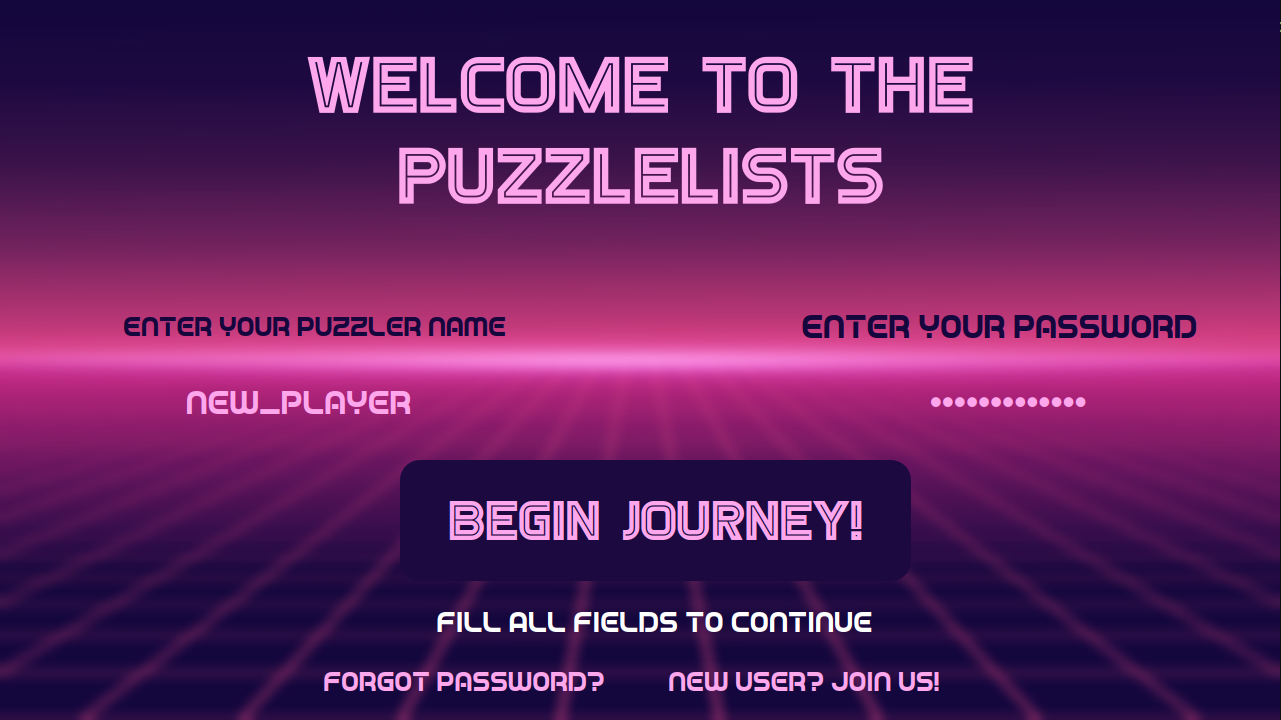
\includegraphics[width=0.8\textwidth]{welcome_screen.png}
    \caption{Login Screen}
\end{figure}

\begin{figure}[H]
    \centering
    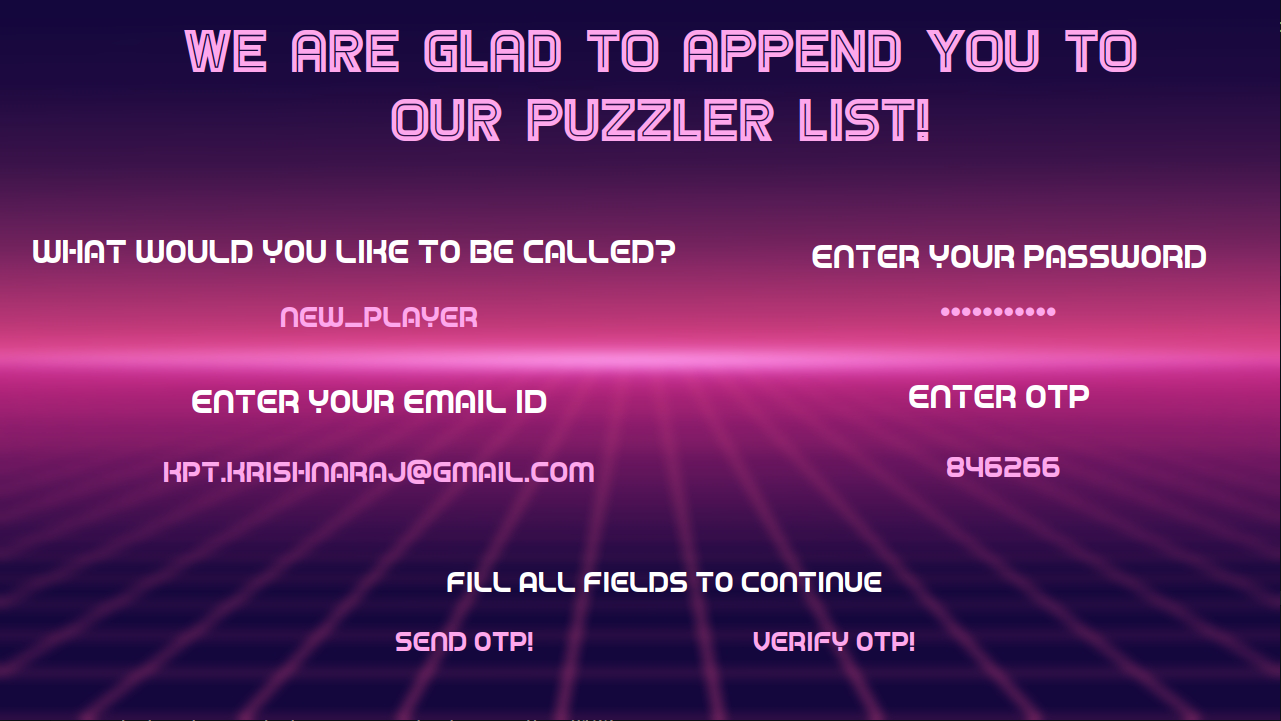
\includegraphics[width=0.8\textwidth]{new_user.png}
    \caption{Register Screen}
\end{figure}

\begin{figure}[H]
    \centering
    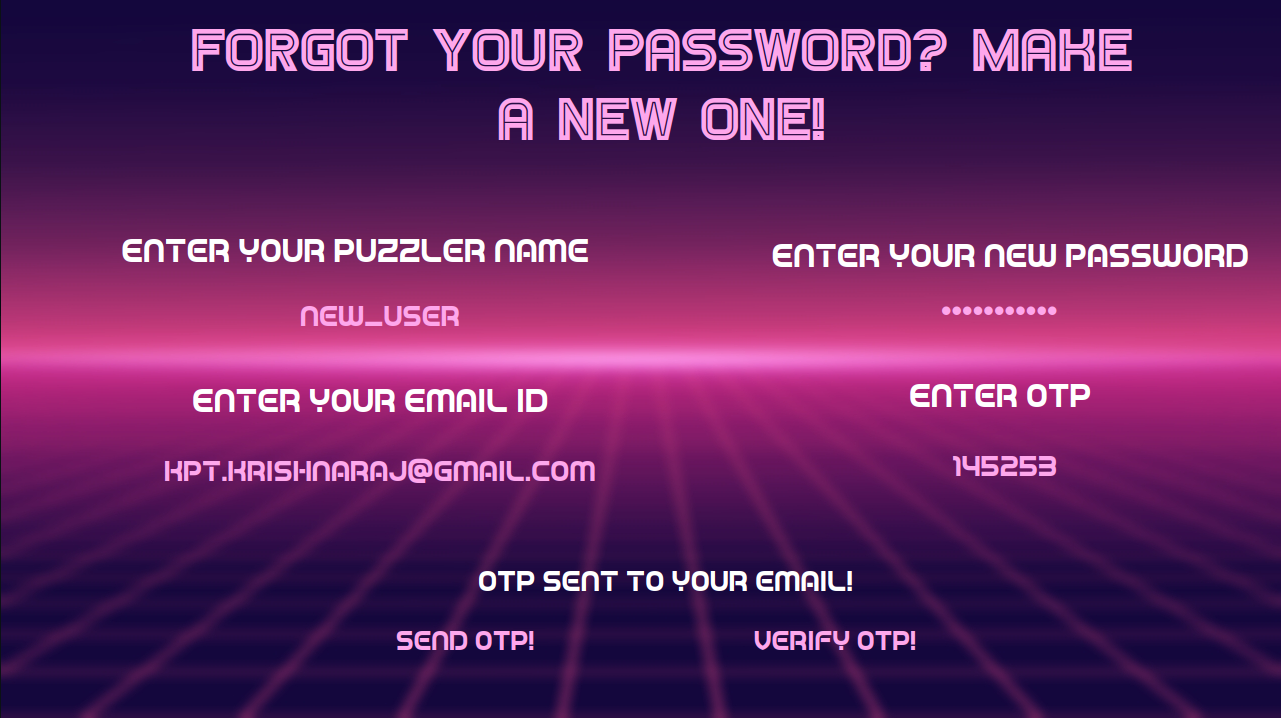
\includegraphics[width=0.8\textwidth]{forgot_password.png}
    \caption{Forgot Password Screen}
\end{figure}

\begin{figure}[H]
    \centering
    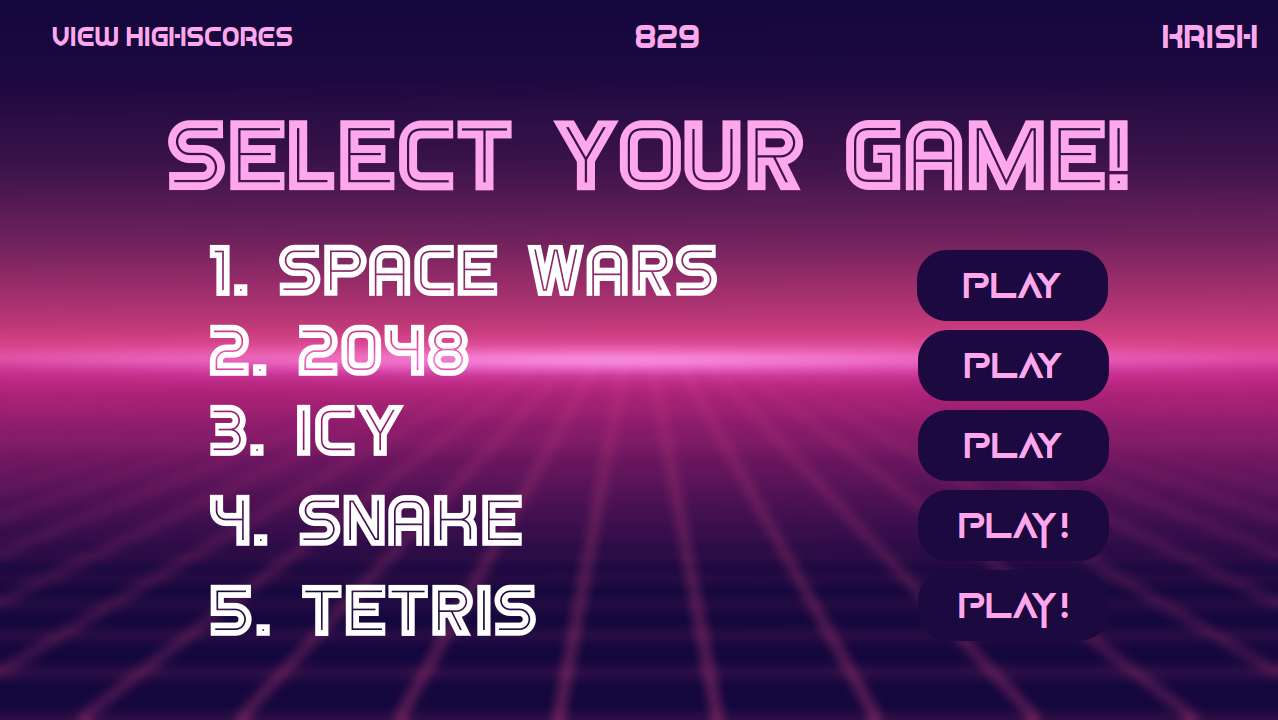
\includegraphics[width=0.8\textwidth]{choose_game.png}
    \caption{Home Screen}
\end{figure}cd 

\begin{figure}[H]
    \centering
    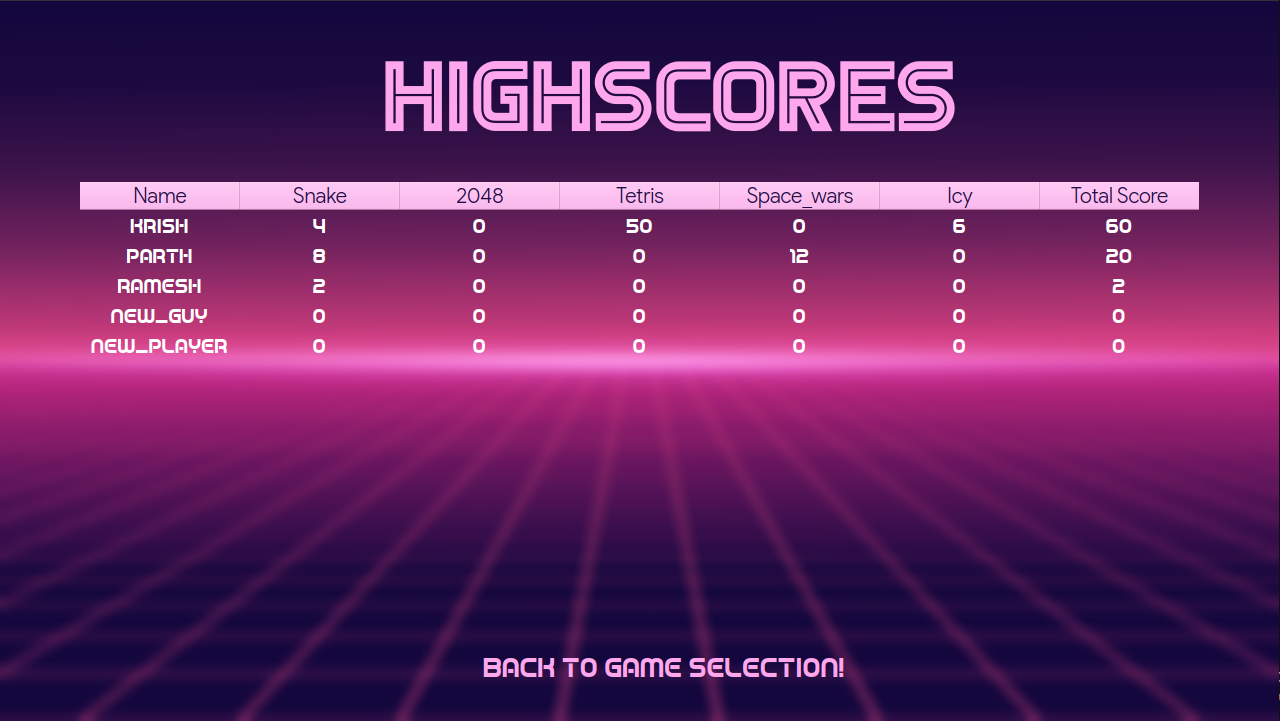
\includegraphics[width=0.8\textwidth]{highscores.png}
    \caption{Highscores Screen}
\end{figure}

\begin{figure}[H]
    \centering
    \includegraphics[width=0.8\textwidth]{space_wars-0.png}
    \caption{Space Wars Screen}
\end{figure}

\begin{figure}[H]
    \centering
    \includegraphics[width=0.8\textwidth]{tetris.png}
    \caption{Tetris}
\end{figure}

\begin{figure}[H]
    \centering
    
\includegraphics[width=0.8\textwidth]{snake.png}
    \caption{Snake}
\end{figure}

\begin{figure}[H]
    \centering
    \includegraphics[width=0.8\textwidth]{icy.png}
    \caption{Icy}
\end{figure}

\begin{figure}[H]
    \centering
    
\includegraphics[width=0.8\textwidth]{2048.png}
    \caption{2048}
\end{figure}

\section{Conclusion:}
In conclusion, Puzzelist is an entertaining and challenging game arcade that showcases the versatility and fun of Python programming. The use of PyQT, Pygame, NumPy and MariaDB libraries has enabled us to create an engaging and interactive gaming experience while ensuring the security and integrity of user data. The project can be further extended by adding more games, improving the graphics and sound, and enhancing the overall user experience.

\section{References:}
\begin{enumerate}
    \item PyQT documentation: https://www.riverbankcomputing.com/static/Docs/PyQt5/
    \item Pygame documentation: https://www.pygame.org/docs/
    \item NumPy documentation: https://numpy.org/doc/   
\end{enumerate}


\end{document}